\documentclass[letterpaper,12pt]{article}
\usepackage[utf8]{inputenc}
\usepackage{amsmath}
\usepackage{amsfonts}
\usepackage{amssymb}
\usepackage{graphicx}
\usepackage{hyperref}
\usepackage{enumerate}
\usepackage[margin=1in]{geometry}

\newcommand{\di}{\displaystyle}
\newcommand{\uu}{\mathbf{u}}
\newcommand{\vv}{\mathbf{v}}
\newcommand{\dotp}{\boldsymbol{\cdot}}
\newcommand{\R}{\mathbb{R}}
\newcommand{\e}{\mathbf{e}}

%opening
\title{Math H53 Fall 2012: On covectors and bivectors}
\author{Sean Fitzpatrick}

\begin{document}

\maketitle

\begin{abstract}
We give a geometric description of the dual vectors, also known as covectors, that are defined as linear functionals on a given vector space $V$. We also expand on the algebraic construction of the bivectors which appear in Assignment \#4. This latter description may be helpful to some of you, since it explains how to think of bivectors as matrices. However, if you find it too abstract, you are free to ignore it.
\end{abstract}

On the your second assignment, we introduced the idea of a linear functional on a vector space $V$: a linear map $\varphi:V\to \R$. We saw that when $V=\R^n$, with vectors identified with column vectors, we can identify the elements of $V^*$ - which are also commonly referred to as covectors or dual vectors - as row vectors. The pairing $\langle \varphi, \vv\rangle = \varphi(\vv)$ can then be viewed as matrix multiplication: a $1\times n$ row vector multiplied by an $n\times 1$ column vector returns a number (a ``$1\times 1$'' matrix, if you will). This is simply the observation that for any column vectors $\uu,\vv\in \R^n$, we have
\[
\uu\dotp\vv = \uu^T\vv,
\]
where $\uu^T$ denotes the transpose of $\uu$ (together with our earlier observation that every linear functional can be given in terms of taking the dot product with some fixed vector).

This point of view is somewhat successful in giving us a more concrete understanding of what a covector is, but doesn't quite let us picture one. Here is a more visual description: the covector $\varphi\in V^*$ dual to a given vector $\uu\in V$ can be pictured as a family of parallel planes whose normal vector is $\uu$. (Note that if $V$ is $n$-dimensional, then these are $(n-1)$-dimensional planes.) The magnitude of $\varphi$ corresponds to the density of the parallel planes: if $\lVert\varphi\rVert$ is large, then the planes will be spaced close together, while if $\lVert\varphi\rVert$ is small, the planes will be farther apart.

Why is this a good geometric picture for a covector? Well, given a vector $\vv\in V$, we need to describe the pairing between $\varphi$ and $\vv$. The pairing here is a simple one: picture $\vv$ as an arrow (in fact, as a {\em literal} arrow - the kind you would shoot from a bow), and picture $\varphi$ as a piece of plywood, or some other sort of layered material. The pairing $\varphi(\vv)$ is then visualized as the number of planes that $\vv$ passes through when it is ``shot'' in. Keep in mind, however, that in this picture, the orientation of the planes, and the angle at which $\vv$ enters, are fixed in advance. (We want $\vv$ to have a particular magnitude and direction, after all.) So the number of planes that $\vv$ passes through depends on the length of the arrow ($\lVert\vv\rVert$), how closely together the planes are spaced ($\lVert\varphi\rVert$) and the angle of $\vv$ relative to the planes. (If $\vv$ is parallel to the planes, it won't pass through any of them, and $\vv$ passes through the maximum number of planes if $\vv$ is orthogonal to the planes.) The picture is something like this:
\begin{center}
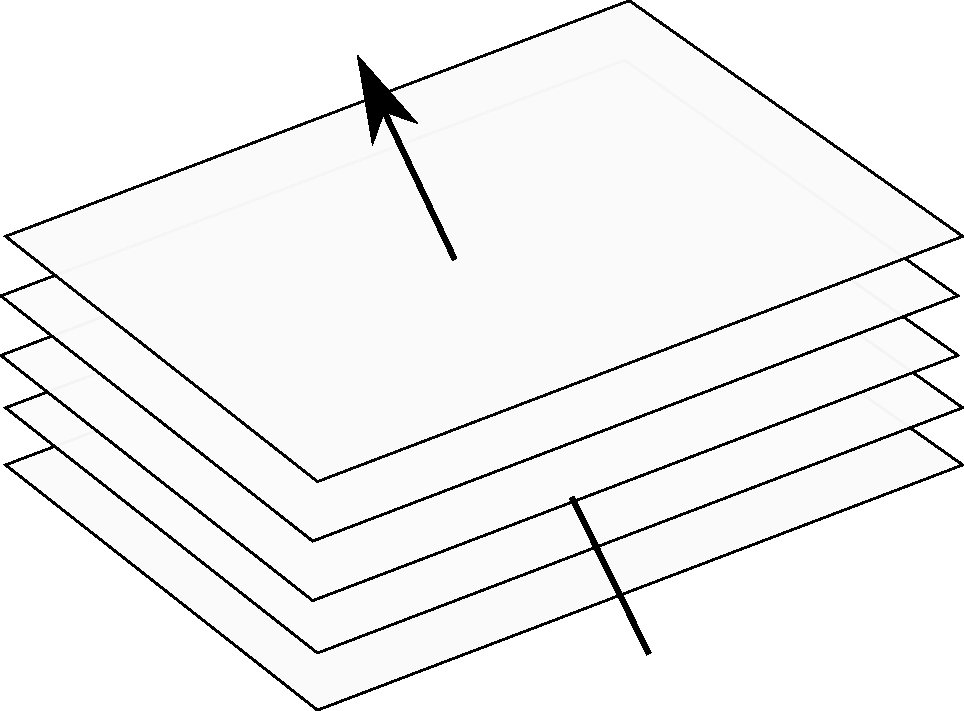
\includegraphics[width=4in]{covector.pdf}
\end{center}
Now, on the fourth assignment, I've introduced something called a bivector, which is written symbolically as $\uu\wedge\vv$, and visualized as the parallelogram spanned by $\uu$ and $\vv$, together with information about how that parallelogram is oriented in space. That's about as good as we can do in terms of visualization, but we can perhaps clarify the algebra a little bit.

When the wedge product is introduced in an abstract algebra setting, it's defined in terms of another product, called a {\em tensor product}. In algebra, a tensor product is used to build bigger vector spaces out of smaller ones. \footnote{This is one option out of several. Another is to take the Cartesian product of vector spaces, and add ordered pairs component-wise - just like we do when we define the two-dimensional space $\R^2$ as the Cartesian product $\R\times\R$. Note that the dimension of $V\times W$ will be the {\em sum} of the dimensions of $V$ and $W$, while the dimension of the tensor product $V\otimes W$ is the {\em product} of the dimensions.}
If $V$ is a vector space with a basis $\{\e_1,\ldots,\e_n\}$ and $W$ is another vector space with a basis $\{\mathbf{f}_1,\ldots, \mathbf{f}_m\}$, we can define a new vector space $V\otimes W$, the tensor product of $V$ and $W$, whose basis vectors are of the form $\e_i\otimes\mathbf{f}_j$, for $1\leq i\leq n$ and $1\leq j\leq m$. The tensor product is required to be linear in both factors:
\begin{align*}
\uu\otimes(c\vv) = (c\uu)\otimes\vv = c(\uu\otimes\vv) &\text{ for all } \uu\in V, \vv\in W, c\in \R\\
\uu\otimes(\vv\otimes\mathbf{w}) = \uu\otimes\vv+\uu\otimes\mathbf{w} &\text{ for all } \uu\in V, \vv,\mathbf{w}\in W\\
(\uu+\vv)\otimes\mathbf{w} = \uu\otimes\mathbf{w}+\vv\otimes\mathbf{w} &\text{ for all } \uu,\vv\in V, \mathbf{w}\in W
\end{align*}
Note that there isn't any sort of commutativity property for the tensor product. In fact, even if $W=V$ (so we're considering $V\otimes V$), there is no relationship between $\e_i\otimes\e_j$ and $\e_j\otimes\e_i$. Notice also that the total number of basis vectors in $V\otimes W$ is $nm$ (so in particular $V\otimes V$ has dimension $n^2$). This seems very abstract and weird, but in fact, tensors can be associated with some very familiar objects: matrices. A general element of $V\otimes W$ is going to be of the form
\[
\psi = \sum_{i=1}^n\sum_{j=1}^m a_{ij}\e_i\otimes \mathbf{f}_j,
\]
where the $a_{ij}$ are real numbers, so we can associate the element $\psi$ with the $n\times m$ matrix whose entries are the numbers $a_{ij}$.

Now, this means that we can associate each element of $V\times V$ with an $n\times n$ matrix. (Notice that as usual, this association depends on a choice of basis.) Among all of the matrices are the so-called anti-symmetric matrices. A matrix is anti-symmetric if
\[
A^T = -A,
\]
where $A^T$ denotes, as usual, the transpose of $A$ (which will again be an $n\times n$ matrix). For example, the matrix
\[
A = \begin{bmatrix}
0 & 1 & 2\\
-1 & 0 & -3\\
-2 & 3 & 0
\end{bmatrix}
\]
is an antisymmetric $3\times 3$ matrix. (Notice that since $a_{ij} = -a_{ji}$ we must have zeros down the main diagonal.) It turns out that the bivectors are simply those tensor products whose corresponding matrix is antisymmetric. In fact, we can define the wedge product in terms of the tensor product: given vectors $\uu,\vv\in V$, we set
\[
\uu\wedge\vv = \frac{1}{2}\left(\uu\otimes \vv -\vv\otimes\uu\right).
\]
This product inherits the linearity of the tensor product, and is also anti-commutative by construction. Finally, let us note that it is possible to consider higher tensor products, including spaces such as $V\otimes V\otimes V$ by insisting that the tensor product be associative. If we want to think of an element $\uu\otimes\vv\otimes\mathbf{w}$ in terms of our original vector space $V$, we can imagine that each element is identified with a {\em three-dimensional} array of numbers $a_{ijk}$, and so on.
\end{document}
